\chapter{Lab Copy on-write:写时复制实验}
\begin{introduction}
    \item 实现写时复制的 Fork 系统调用
    \item 写时复制的好处
\end{introduction}

写时复制( COW )机制是操作系统中一种常见的惰性机制,在很多场景下可以提供较好的性能和比物理资源多很多的虚拟资源量,因而机制在内存管理中使用较多。实现 COW 机制需要我们将前几个实验的涉及的概念(进程、分页和中断)融会贯通,从这个实验开始,我们的工作将遍及 xv6 内核的各个部分。

\section{实现写时复制的 Fork 系统调用}

我们早在第三章 Lab Utilities 中就已经接触了 xv6 中用于生成子进程的系统调用 fork ,该系统调用由于其实用的设计被后世的类 Unix 系统一直沿用,可谓 Unix v6 留下的宝贵遗产。在原始的 xv6 的实现中, fork 会将父进程的所有页面完整地复制到一份,映射到子进程中。然而很多时候,子进程只会读取这些页面的内容,而不会写入这些页面。为了节约内存的实际用量,我们可以在子进程(或父进程)真正需要写入页面时才分配新的页面并进行数据的复制,这种机制被称为 COW fork 。

在本实验中,我们需要改进原先 xv6 的 fork ,使其使用 COW 机制。为了验证实现的正确性, xv6 提供了 \lstinline{cowtest} 用户程序供验证。

由于这个实验涉及到将进程、分页和中断综合起来,故整个实现较为困难。我们首先修改物理内存分配器,由于 COW 中一个物理页面不仅被映射给一个页表,故而我们需要一个数据结构维护其引用的数量,故而在 \lstinline{kalloc.c} 中添加以下变量:
\begin{lstlisting}[language=C]
......
struct spinlock reflock;
uint8 referencecount[PHYSTOP/PGSIZE];
......
\end{lstlisting}

然后在初始化内存管理器的 \lstinline{kinit} 中添加初始化引用计数锁的语句:
\begin{lstlisting}[language=C]
void
kinit()
{
  initlock(&kmem.lock, "kmem");
  initlock(&reflock, "ref");
  freerange(end, (void*)PHYSTOP);
}
\end{lstlisting}

之后更改释放物理页面的代码,使得每次释放仅将引用计数减一,直到引用计数为 0 后才真正释放页面:
\begin{lstlisting}[language=C]
void
freerange(void *pa_start, void *pa_end)
{
  char *p;
  p = (char*)PGROUNDUP((uint64)pa_start);
  for(; p + PGSIZE <= (char*)pa_end; p += PGSIZE)
  {
    acquire(&reflock);
    referencecount[(uint64)p / PGSIZE] = 0;
    release(&reflock);
    
    kfree(p);
  }
}
\end{lstlisting}

完成修改物理内存分配器的准备工作后,再考虑完成 COW 的前半部分:将父进程的页面映射给子进程,并给父进程和子进程的页表设为只读。

首先找到 fork 系统调用的实现,从 \lstinline{sysproc.c} 中的 \lstinline{sys_fork} 开始,找到 \lstinline{proc.c} 中的 \lstinline{fork()} 。我们发现, \lstinline{fork()} 中用于拷贝父进程页面到子进程的代码如下:
\begin{lstlisting}[language=C]
int
fork(void)
{
......
  // Copy user memory from parent to child.
  if(uvmcopy(p->pagetable, np->pagetable, p->sz) < 0){
    freeproc(np);
    release(&np->lock);
    return -1;
  }
......
\end{lstlisting}

其中调用了 \lstinline{uvmcopy} ,找到 \lstinline{uvmcopy} 在 \lstinline{vm.c} 中的实现:
\begin{lstlisting}[language=C]
int
uvmcopy(pagetable_t old, pagetable_t new, uint64 sz)
{
......
  for(i = 0; i < sz; i += PGSIZE){
......
    pa = PTE2PA(*pte);
    flags = PTE_FLAGS(*pte);
    if((mem = kalloc()) == 0)
      goto err;
    memmove(mem, (char*)pa, PGSIZE);
    if(mappages(new, i, PGSIZE, (uint64)mem, flags) != 0){
      kfree(mem);
      goto err;
    }
  }
......
}
\end{lstlisting}

其确实尝试分配页面并拷贝数据。

对 \lstinline{uvmcopy} 进行修改,使用 \lstinline{mappages} 只映射页面、增加引用计数并修改权限为只读,而不分配页面:
\begin{lstlisting}[language=C]
int
uvmcopy(pagetable_t old, pagetable_t new, uint64 sz)
{
......
  for(i = 0; i < sz; i += PGSIZE){
......
    *pte &= ~(PTE_W);
    *pte |= PTE_COW;
    pa = PTE2PA(*pte);
    flags = PTE_FLAGS(*pte);
    if(mappages(new, i, PGSIZE, (uint64)pa, flags) != 0){
      goto err;
    }
    acquire(&reflock);
    referencecount[PGROUNDUP((uint64)pa)/PGSIZE]++;
    release(&reflock);
  }
......
}
\end{lstlisting}
这里使用了分页机制中为软件使用保留的第 8 位作为标志位,若其为 1 ,则说明其为 COW 页。

由于 \lstinline{uvmcopy} 引入了引用计数,在删除页面映射的过程 \lstinline{uvmunmap} 中也要加入对应的操作,从而可以使得引用计数保持正确:
\begin{lstlisting}[language=C]
extern struct spinlock reflock;
extern uint8 referencecount[PHYSTOP/PGSIZE];
void
uvmunmap(pagetable_t pagetable, uint64 va, uint64 npages, int do_free)
{
......
    acquire(&reflock);
    referencecount[PGROUNDUP((PTE2PA(*pte)))/PGSIZE]--;
    if(do_free && referencecount[PGROUNDUP((PTE2PA(*pte)))/PGSIZE] < 1){
      uint64 pa = PTE2PA(*pte);
      kfree((void*)pa);
    }
    release(&reflock);
    *pte = 0;
......
}
\end{lstlisting}

此时就完成了 COW 的前半部分,如果父进程和子进程都在 fork 后没有写入内存,则一切相安无事;而若其中一个进程尝试写入内存,则会引发页面权限错误,从而产生一个中断最终调用 \lstinline{usertrap()}。

查阅手册 \textit{The RISC-V Instruction Set Manual: Volume II: Privileged Architecture}  \footnote{\url{https://riscv.org/wp-content/uploads/2017/05/riscv-privileged-v1.10.pdf}} ,得知写页面权限造成的错误引发的中断会使得 SCAUSE 寄存器被设为 12 或 15 ,且 STVAL 寄存器中会存储违反权限的虚拟内存地址。我们通过 \lstinline{riscv.h} 中提供的读寄存器函数获取这两个寄存器的内容后,就可以稍作判断,若违例访问确为 COW 引起的,就可以分配页面、复制数据并进行释放页面、修改页面权限和标志等后续工作,否则杀死进程并进行善后工作。具体笔者在 \lstinline{trap.c} 中的实现如下:
\begin{lstlisting}[language=C]
void
usertrap(void)
{
......
  } else if (r_scause() == 12 || r_scause() == 15){
    // deal with cow pages
    pte_t *pte;
    uint64 pa, va;
    uint flags;
    char *mem;

    va = r_stval();
    if(va >= MAXVA)
    {
      p->killed = 1;
      exit(-1);
    }
      
    if((pte = walk(p->pagetable, va, 0)) == 0)
    {
      p->killed = 1;
      exit(-1);
    }
    if((*pte & PTE_V) == 0)
    {
      p->killed = 1;
      exit(-1);
    }
    if((*pte & PTE_COW) == 0)
    {
      p->killed = 1;
      exit(-1);
    }

    pa = PTE2PA(*pte);
    flags = PTE_FLAGS(*pte) | PTE_W;
    flags &= ~(PTE_COW);

    if((mem = kalloc()) == 0)
    {
      p->killed = 1;
      exit(-1);
    }
    memmove(mem, (char*)pa, PGSIZE);
    uvmunmap(p->pagetable, PGROUNDDOWN(va), 1, 1);
    if(mappages(p->pagetable, PGROUNDDOWN(va), PGSIZE, (uint64)mem, flags) != 0){
      kfree(mem);
      panic("cowhandler: mappages failed");
    }
  }
......
  usertrapret();
}
\end{lstlisting}

此时 COW fork 的机制基本完成,但 xv6 的实验手册还提醒我们,需要修改 \lstinline{copyout()} 使得其能够适应 COW 机制:因为 \lstinline{copyout()} 是在内核态修改用户态的页面内存,故而不会引发从用户态来的违例访问,因此需要我们做特殊处理。查看 \lstinline{vm.c} 中 \lstinline{copyout()} 的实现,相关代码如下:
\begin{lstlisting}[language=C]
int
copyout(pagetable_t pagetable, uint64 dstva, char *src, uint64 len)
{
  uint64 n, va0, pa0;

  while(len > 0){
    va0 = PGROUNDDOWN(dstva);
    pa0 = walkaddr(pagetable, va0);
    if(pa0 == 0)
      return -1;
    n = PGSIZE - (dstva - va0);
    if(n > len)
      n = len;
    memmove((void *)(pa0 + (dstva - va0)), src, n);

    len -= n;
    src += n;
    dstva = va0 + PGSIZE;
  }
  return 0;
}
\end{lstlisting}

我们判断一个页面是否为 COW 页面使用的是上面提到的 \lstinline{#define PTE_COW (1L << 8)} 标志位,然后使用与处理违例访问相似的方法,进行分配页面、复制数据并进行释放页面、修改页面权限和标志等后续工作。笔者的实现如下:
\begin{lstlisting}[language=C]
int
copyout(pagetable_t pagetable, uint64 dstva, char *src, uint64 len)
{
  uint64 n, va0, pa0;
  pte_t *pte;
  while(len > 0){
    va0 = PGROUNDDOWN(dstva);
    pa0 = walkaddr(pagetable, va0);
    if(dstva >= MAXVA)
      return -1;
    pte = walk(pagetable, va0, 0);
    if(pa0 == 0)
      return -1;
    n = PGSIZE - (dstva - va0);
    if(n > len)
      n = len;
    if (*pte & PTE_COW)
    {
      uint flags;
      char *mem;
      flags = PTE_FLAGS(*pte) | PTE_W;
      flags &= ~(PTE_COW);
      if((mem = kalloc()) == 0)
      {
        return -1;
      }
      memmove(mem, (char*)pa0, PGSIZE);
      uvmunmap(pagetable, va0, 1, 1);
      if(mappages(pagetable, va0, PGSIZE, (uint64)mem, flags) != 0)
      {
        kfree(mem);
        panic("copyout: mappages failed");
      }
    }
    pa0 = walkaddr(pagetable, va0);
    memmove((void *)(pa0 + (dstva - va0)), src, n);

    len -= n;
    src += n;
    dstva = va0 + PGSIZE;
  }
  return 0;
}
\end{lstlisting}

至此,整个 COW fork 机制便实现完成了。

\paragraph*{实验结果} 在完成 Lab Copy on-write 中的所有实验后,根据 MIT 6.S081 的传统,需要在实验目录下创建一个名为 \lstinline{time.txt} 文本文件,其中只包含一行,为完成该实验的小时数。然后在终端中执行 \lstinline{make grade} ,即可对整个实验进行自动评分,笔者的结果如下:
\begin{figure}[H]
  \centering
  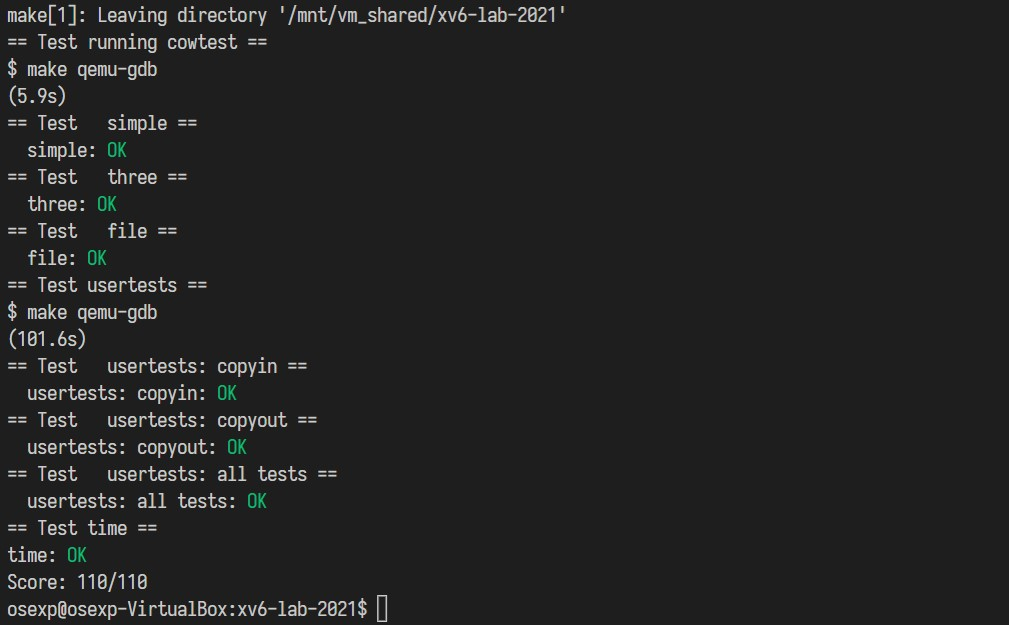
\includegraphics[width=0.8\textwidth]{cow_grade.jpg}
  \caption{ Lab Copy on-write 的测评结果}
\end{figure}
可见测试全部通过,得分为满分。


\section{小结:写时复制(和其它惰性机制)的讨论}

软件工程中有一句重要的论述,出自 Butler Lampson 之手: \textit{All problems in computer science can be solved by another level of indirection.} 通过增加一层中间层,就有了可以引入一些优化机制的空间,这一点不仅在操作系统中极其常见,在其它软件工程的实践中也比比皆是。

在我们本次实验的 COW fork 的例子中,不直接分配页面,而是通过 COW 机制惰性地在程序需要时再分配页面,至少带来了如下几点好处:
\begin{enumerate}
    \item 由于初次 fork 无需真正复制内存, fork 执行地更快
    \item 对于计算密集型的任务,可能子进程无需写内存,故而可以超出物理内存的限制而执行更多的进程
    \item 由于程序局部性原理的存在,即便子进程需要对某些页面进行写入,存放代码段的页面也是父子进程共享的
    \item 共享的内存页面可以大幅度提高处理器中 cache 的效率,提高速度
\end{enumerate}

事实上, COW 机制除了在内存管理中被使用外,在文件系统乃至操作系统外的软件(如数据库)中,也被用于实现一部分的惰性。惰性机制除了 COW 外,我们熟悉的内存交换机制和一些编程语言中提供的惰性求值等,也是惰性机制的体现。惰性机制的核心在于“按需分配”,从而能够避免资源浪费。

避免资源浪费在大多数情况下已经足够优秀了,但在具有更高性能需求的场景,仅仅避免浪费还不够,它们需要系统能够提前准备好程序恰好需要的资源。所以在现代的软件系统中,除了惰性机制,一些基于启发式算法的预测机制也被引入以提高性能。作为惰性机制的反面,提前预测的机制在预测成功时会带来受益,但预测失败则会造成更大的资源浪费与性能损失。在操作系统的层面上,由于预测失败的惩罚较大,故而更多的优化还是从保守的避免浪费的观点出发。